\section{Experimental Design}

\subsection{Sample Preparation}
Before performing any kind of measurements, we first need to ensure that the sample's quality is as high as possible. This means it should be as close to atomically smooth and free 
from adsorbed contaminants as we can manage. This is achieved by using a combination of Argon ion (\ce{Ar+}) bombardment and annealing of the sample. Progress is qualified by examining 
the low energy electron diffraction (LEED) pattern obtained from the sample. 

The sample used for every trial in this experiment is a 1cm $\times$ 1cm $\times$ 1mm Cu(111) metal square, which was stored in atmosphere in a desiccator . It was transferred into the IPES system 
by means of a sample garage in a load-lock chamber. Once the load-lock was brought down to vacuum the sample was then seated in a holder within the preparation chamber. This holder
is height adjustable and allows for the sample to be aligned with the \ce{Ar+} beam for etching; the holder also contains a button heater which is powered from an external lab bench 
supply, and is used for annealing the sample. \figref{prepchamber} shows the Cu sample seated in the sample holder (centre of viewing window), aligned with the beam from the \ce{Ar+}
gun (top left). 

\begin{figure}[h!]
    \centering
    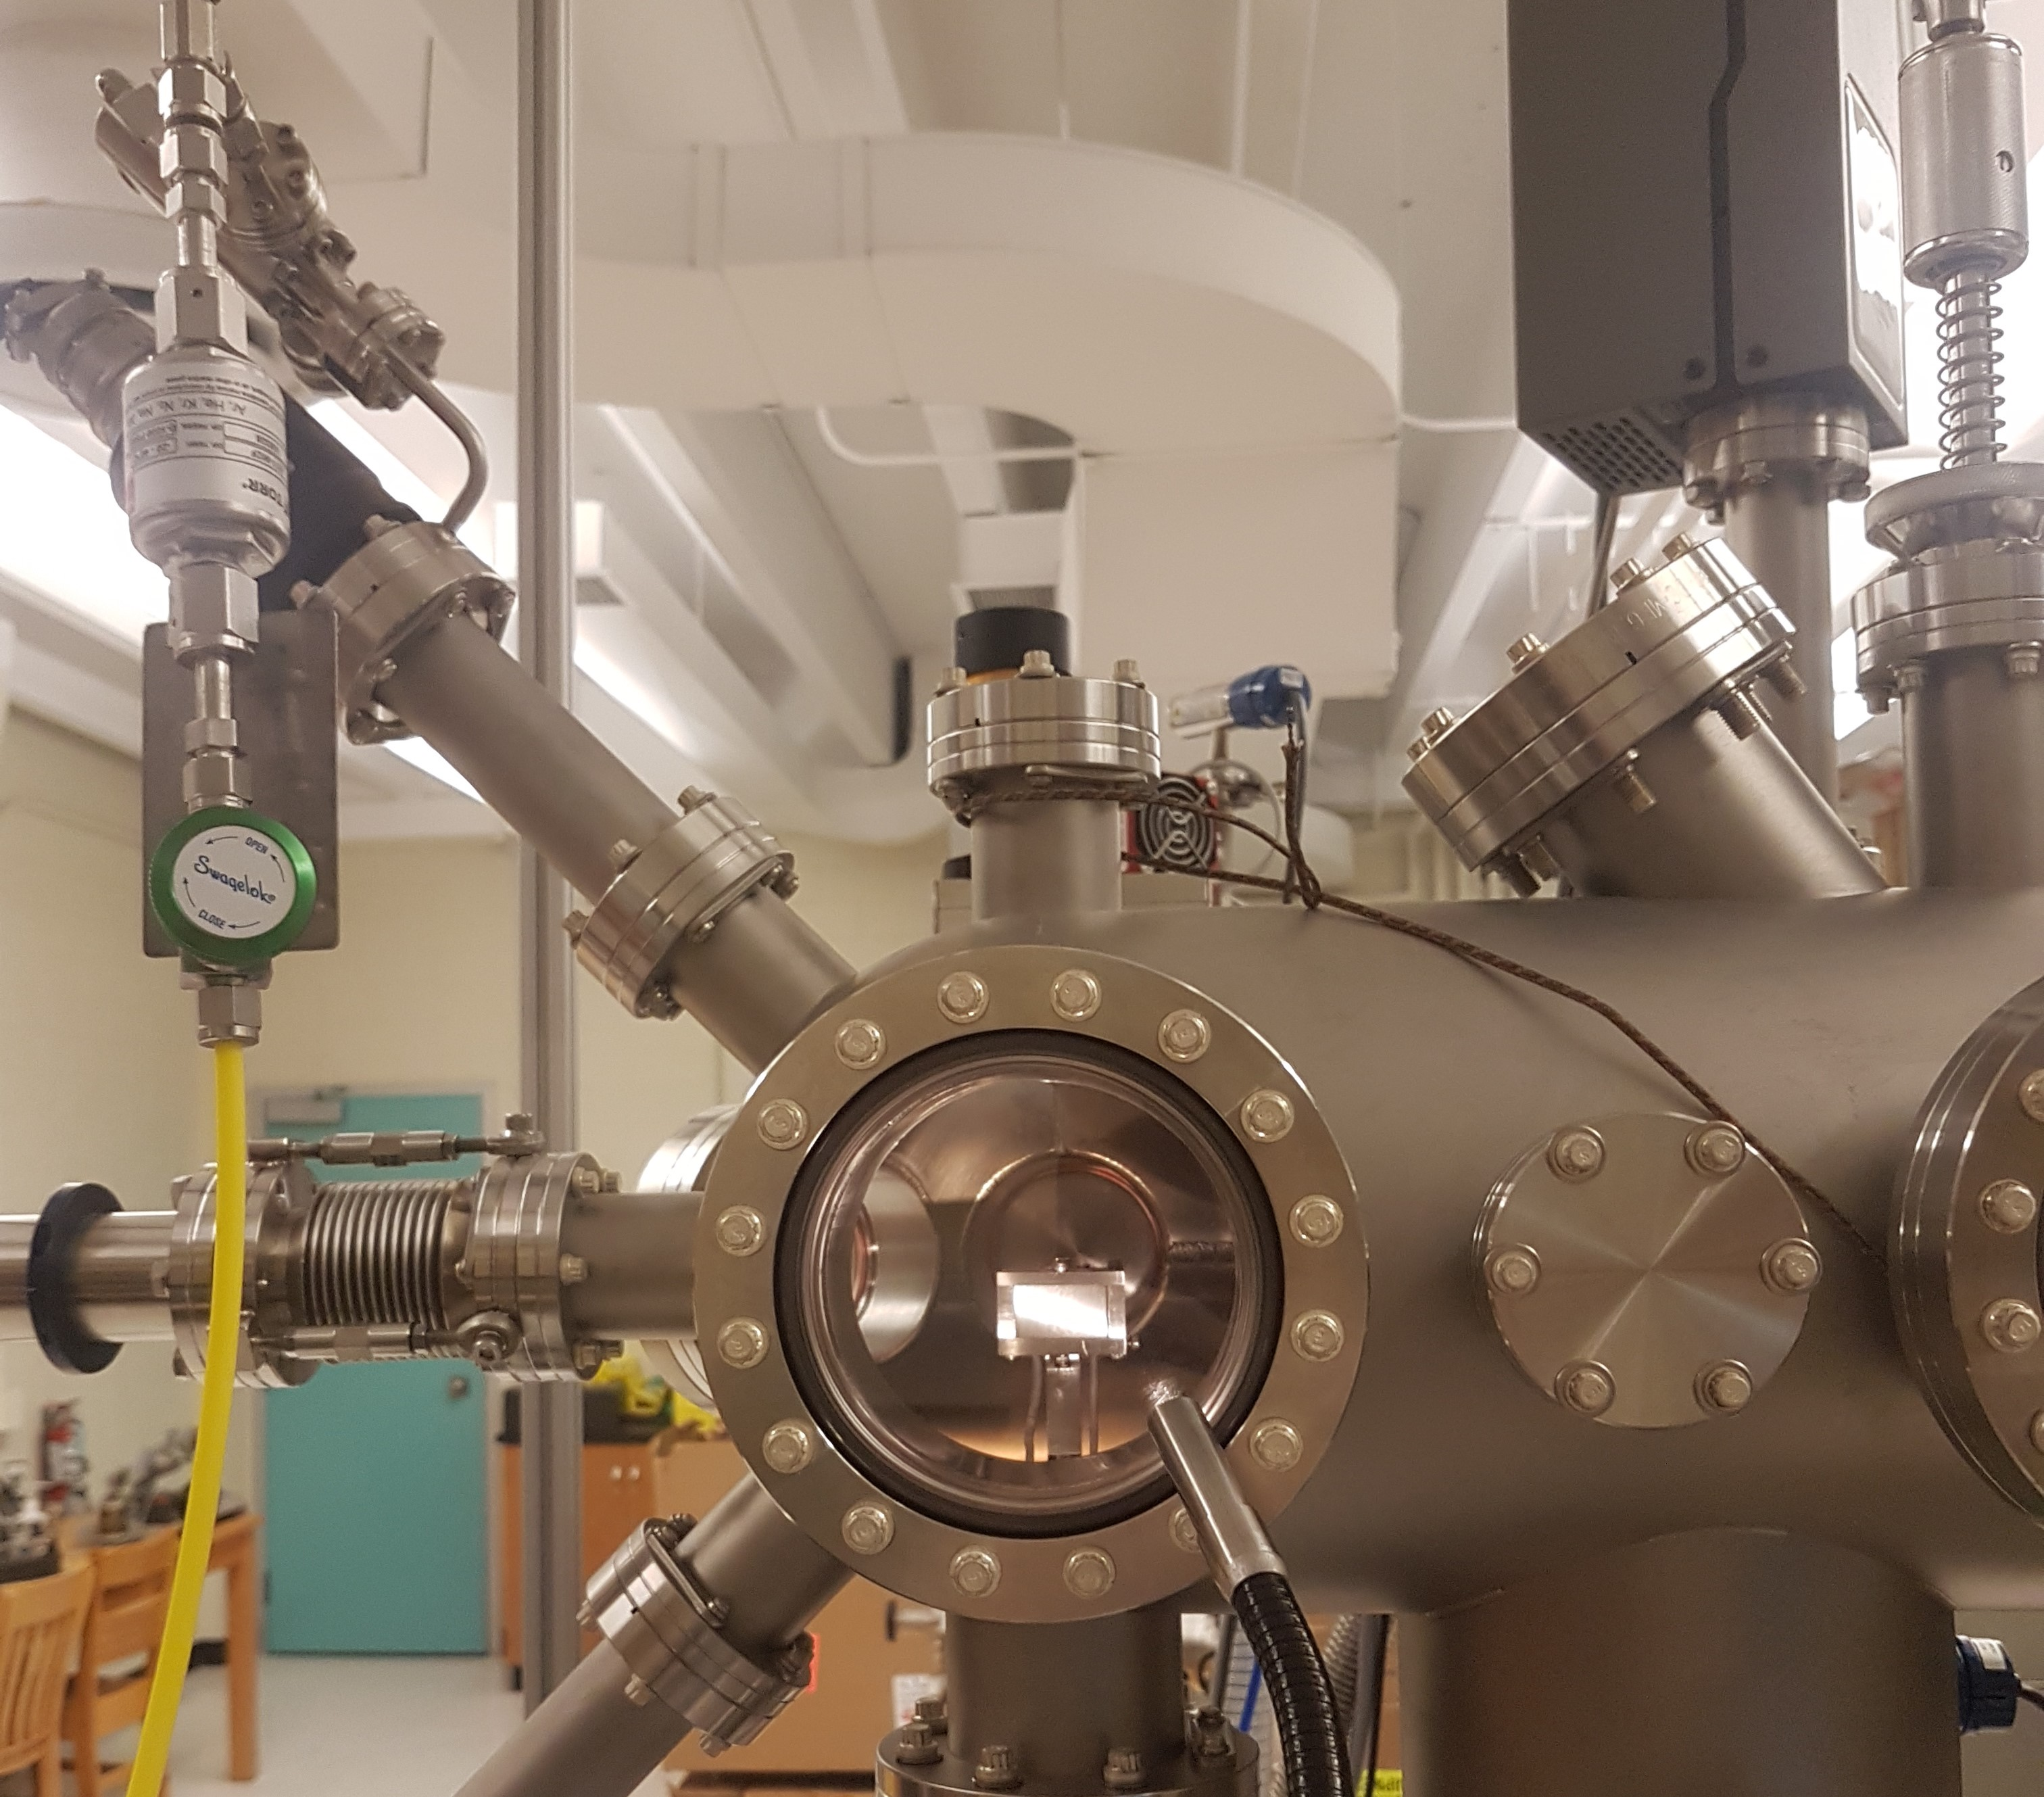
\includegraphics[scale=0.08]{Figs/prep.jpg}
    \caption{Prep chamber set up for \ce{Ar+} etching of Cu sample}
    \label{fig:prepchamber}
\end{figure}

With the sample loaded and aligned, the ion gun was turned on and set up. First the ion current was set to 20mA, then the beam energy was set to 1kV. Once the gun was up to temperature
and outgassing from the heated filament had stopped, Ar could be introduced to the gun to be ionized and accelerated. A needle valve controls the flow of gas into the gun, and it is 
connected to a filter to remove trace gases as the Ar flows from the main cylinder. The pressure of gas was increased until it settled at approximately $1\times10^{-5}$ torr.
The sample was left in this configuration for a full day, after which the gas was turned off and the gun was powered down. The sample was then transferred to the main chamber once the 
pressure of residual Ar in the prep chamber had decreased. Once in the main chamber, it was aligned so that a LEED pattern could be obtained. The sample was then transferred back to the prep chamber and seated in the sample holder for annealing. 

To anneal the sample the button heater was connected to a lab bench power supply by means of a feedthrough in the prep chamber. The current on the supply was set to 4.5A and the temperature
of the sample was monitored using a K-type thermocouple in contact with the heater stage. The temperature of the stage and sample rose slowly over the period of a day, finally 
settling at 450$^\circ$C. Once this temperature was achieved the sample was left to anneal for another full day. The goal of annealing is to heat the sample enough that atoms on the 
surface become mobile allowing for atoms on peaks in the sample to fill in valleys, leading to a smoother surface\cite{robinson2012argon}. The process of obtaining a LEED pattern was 
repeated once the sample had cooled to room temperature, a comparison of LEED patterns for etching with no annealing, and etching with annealing can be seen in \figref{LEED}. The sample
was then left in the main chamber for the next steps of the experiment. 

\begin{figure}[h!]
  \centering
  \subcaptionbox{LEED pattern obtained for Cu(111) sample cleaned using only \ce{Ar+} etching. Spots which are not part of $C_6$ symmetric pattern indicate defects in the surface.}[0.35\linewidth]{\includegraphics[scale=0.07]{Figs/etched.png}}
  \subcaptionbox{LEED pattern for \ce{Ar+} etched and annealed Cu(111). Only the expected $C_6$ pattern is visible indicating a smooth surface free of contaminants.}[0.35\linewidth]{\includegraphics[scale=0.07]{Figs/annealed.png}}
  \caption{Comparison of LEED patterns obtain for Cu(111) during different phases of sample preparation. The only pattern visible at this energy should be a hexagon, reflecting the 
  hexagonal shape of the (111) plane of an FCC lattice.}
  \label{fig:LEED}
\end{figure}

\subsection{Experimental Setup}

Within the main vacuum chamber of the system is where IPES takes place. A sample is loaded into a motorized sample holder with the ability to translate in X, Y, and Z directions 
and to rotate about the central (Z) axis of the chamber. Once mounted the sample is moved to be placed in front of the output of the electron gun. The photodetector tubes, mounted to 
ConFlat bellows, are then brought close to the sample to maximize the solid angle made up by the detectors. The tubes are mutually connected to a gas manifold that allows control 
over whether a tube is pressurized (through the use of valves), and the extent of the pressurization. The manifold is connected to a small bottle of spectroscopy grade acetone, and
a turbopump cart; by opening the needle valve to the acetone bottle the pressure of the tubes can be increased, and by opening a valve to the pump cart it can be decreased allowing 
for fine control over the pressure of the system.

The detectors are connected to a Cremat charge sensitive preamplifier kit\cite{CR-150-R5}, which contain a CR-110-R2.1 preamplifier chip\cite{CR-11X}. This chip has a gain of 1.4V/pC, and is the 
largest gain available from Cremat, it was chosen because of the small charge pulses that come from IPES detections. The connection from the preamp to the detector is done through a 
safe high voltage (SHV) feedthrough which is connected directly to the anode wire. The preamplifier is responsible for converting the current pulse from the anode, caused by the 
Townsend avalanches, into a voltage pulse with signal strength proportional to the input current. The preamp contains an SHV input which is used to bias the detector, and 
an a coax output for the voltage pulse. The output signal is fed into a Cremat Guassian shaping amplifier\cite{CR-160-BOX-R4}, which converts the step-function voltage pulse from 
the preamplifier into a Guassian signal. The shaping amplifiers for both detectors use a CR-200-500ns-R2.1 shaping module, which has a 500ns shaping time and yields a Gaussian pulse
with a FWHM of 1.2$\mu$s\cite{CR-200-X}. A comparison of the two pulses can be seen in \figref{pulses}, which shows the step-function pulse from the preamplifier in yellow, and the 
resulting Gaussian pulse from the shaping amplifier in blue. 

\begin{figure}[h!]
  \centering
  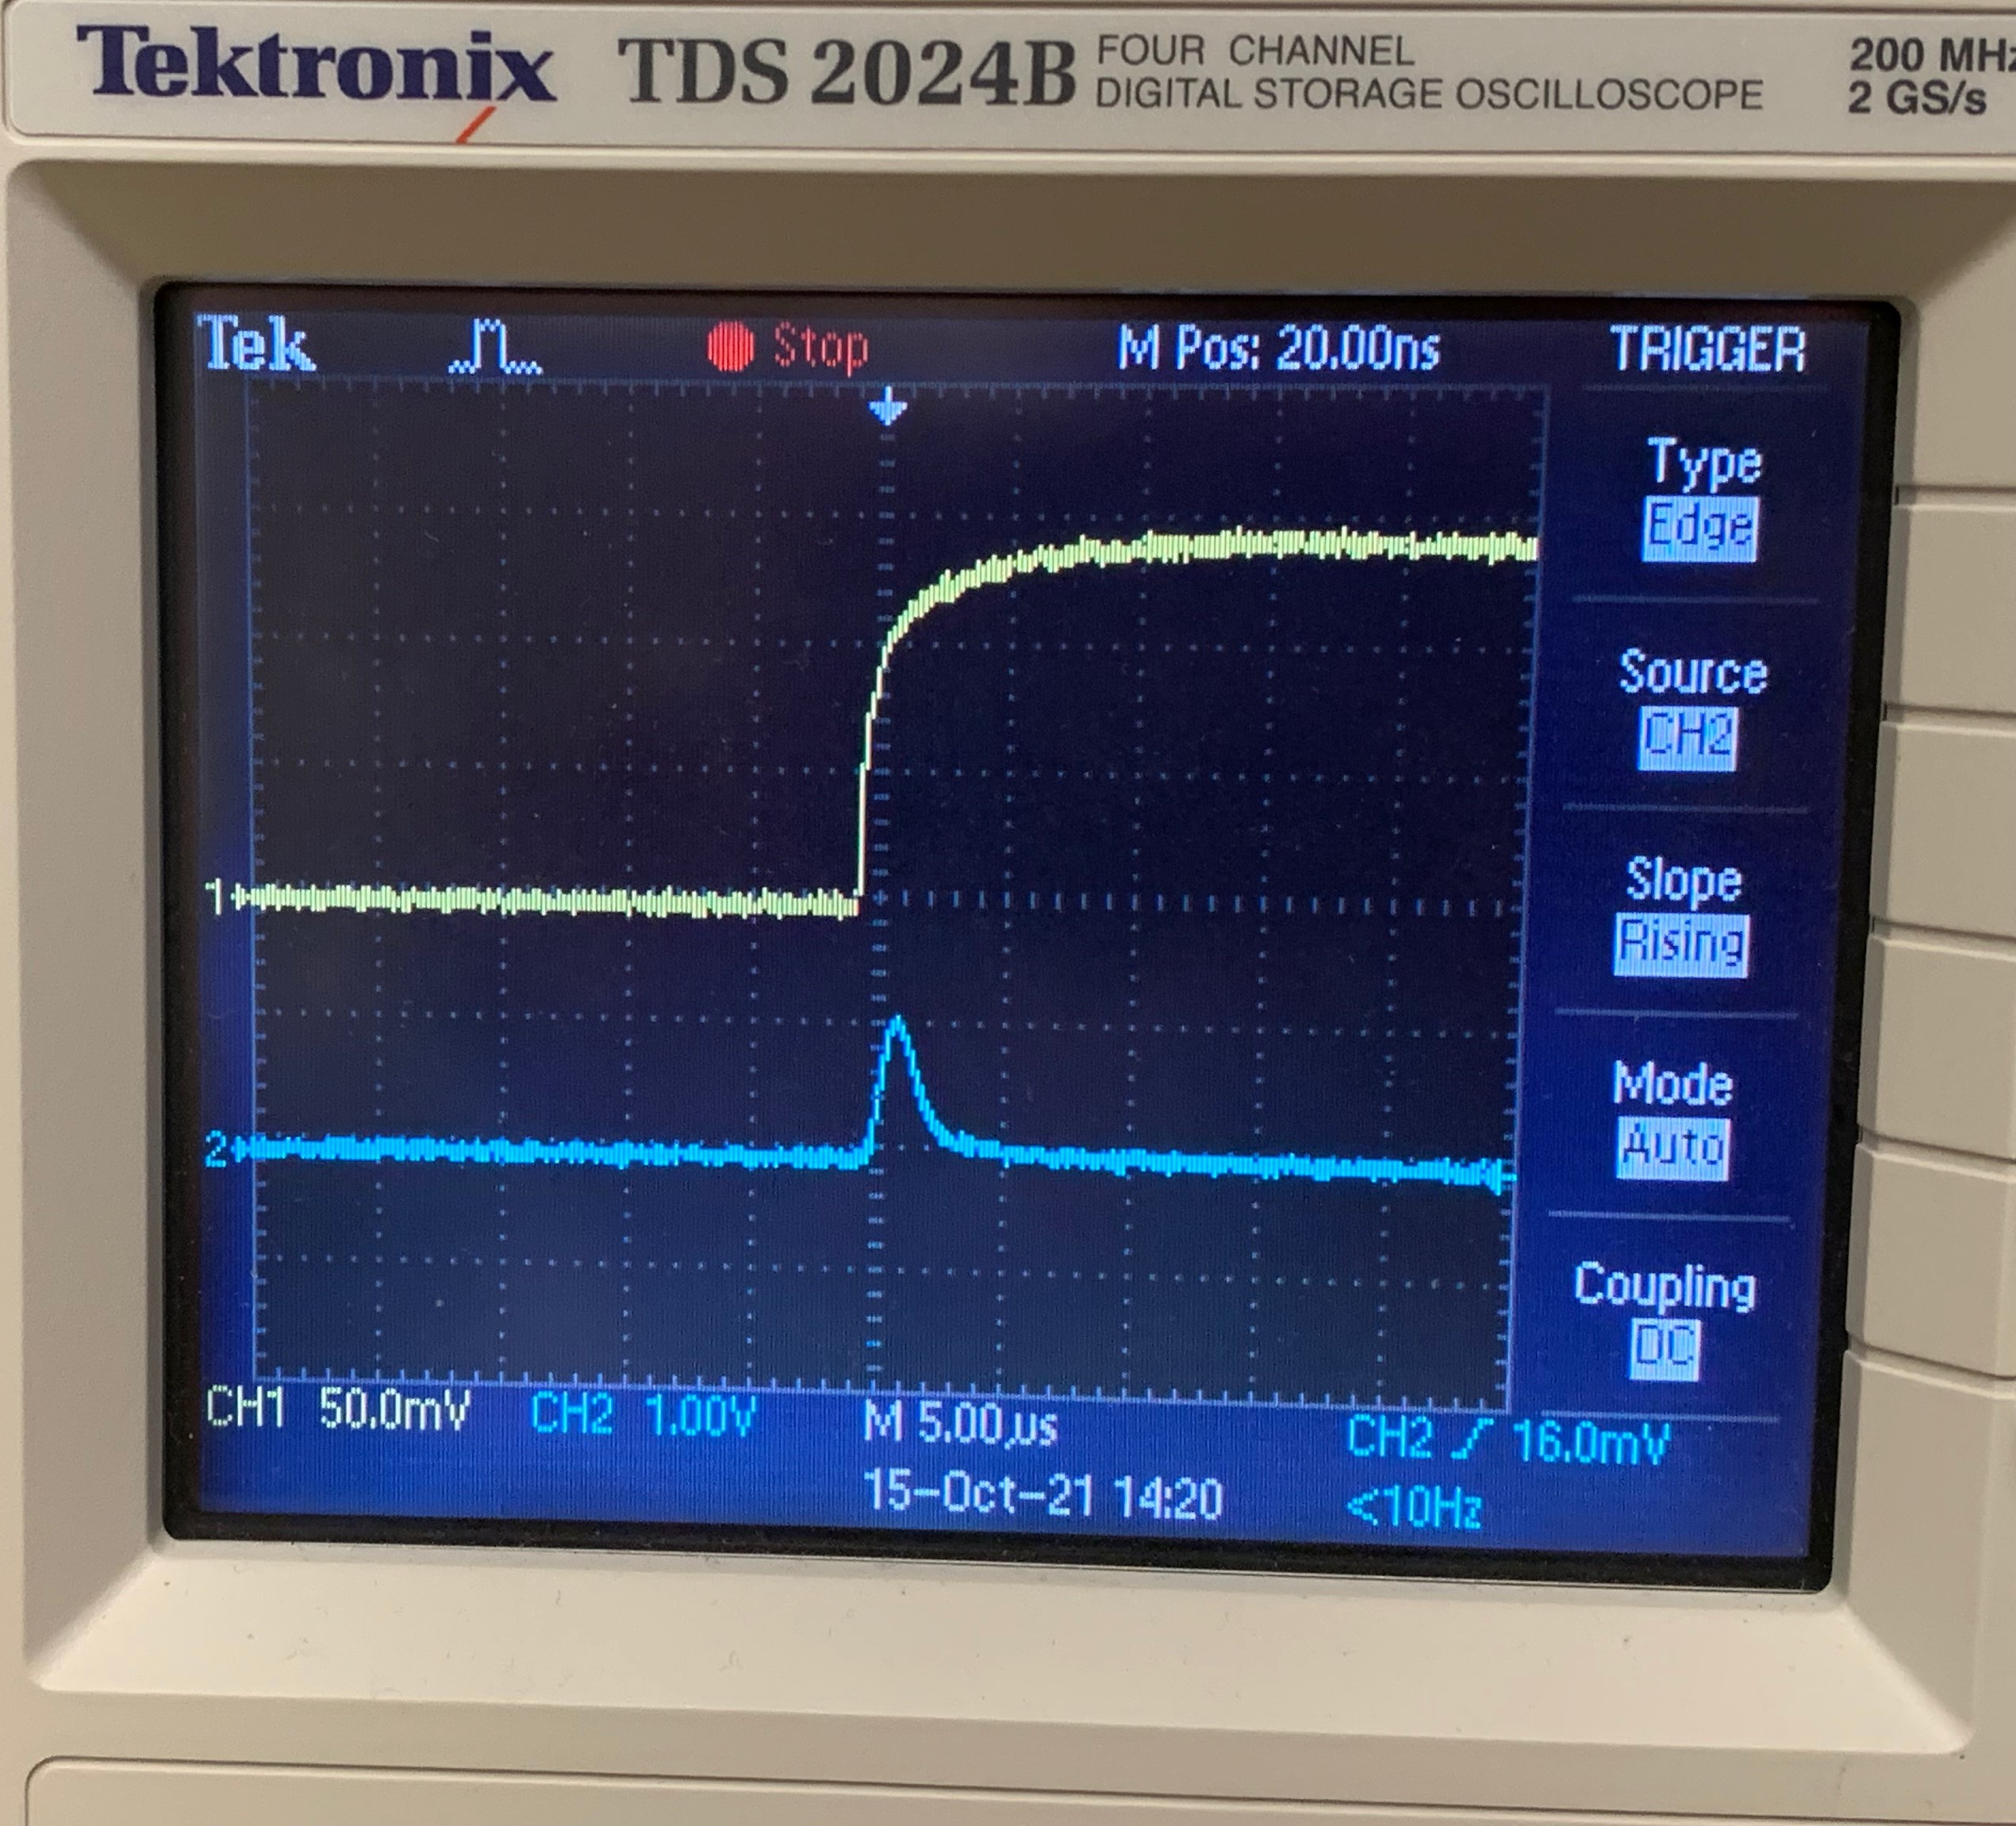
\includegraphics[scale=0.15]{Figs/pulses.png}
  \caption{Preamplifier (yellow) and shaping amplifier (blue) pulses shown on an oscilloscope}
  \label{fig:pulses}
\end{figure}

The output pulses from both shaping amplifiers are fed into two ADC converter inputs on a FAST ComTec multichannel analyzer. The MCA is set up to detect Gaussian input pulses above a certain threshold 
value, which from experimentation was set to 30mV. Most signals with pulse height less than 30mV were found to just be electronic noise cause by the addition of a resistor to the preamplifier
to prevent damage from over-current due to tube breakdown. The MCA keeps a running count of how many pulses above this threshold it detects in a given amount of time, and in addition 
automatically produces a pulse height distribution. The number of counts from the MCA is then finally sent to a computer using LabVIEW. 

\subsection{Procedure}

The general procedure for this experiment is based on the work done by Banik and Shukla, who examined what combination of acetone pressure and anode voltage 
would maximize counts and minimize tube breakdowns\cite{banik2005optimal}. Our experiment started by evacuating the tubes of acetone, which was done because the energy involved from tube breakdown is large
enough to crack the acetone rendering it useless for detecting photons\cite{banik2005optimal}. The tubes were then filled with acetone to the desired pressure. Next the electron gun and 
high voltage power supply were powered on, with 5V being passed to the gun's filament to provide a source of electrons using thermionic emission. A LabVIEW virtual instrument was used 
to control the various components of the experiment. The following is an excerpt from the command file written for the LabVIEW program:

\begin{center}
  \begin{verbatim}
    set;va;300.0;
    set;vb;300.0;
    set;en;15.0;
    measure;gm1;
    measure;gm2;
    measure;6487c;
    set;en;0.0;
    measure;gm1;
    measure;gm2;
    measure;6487c;
  \end{verbatim}
\end{center}

The program starts by setting the bias voltage used for both detectors, in this case using a value of 300V. Next the electron gun is set to emit electron with an energy of 15eV, 
which was chosen simply because it gave a high count rate for the Cu sample used. The program is told to wait 3 seconds before executing the next command which is done to allow the emission of photons from the sample to stabilize and give an accurate impression 
of the count rate. When the waiting period is over the program then runs the MCA for a predetermined amount of time, which was either 30, 15, or 5 seconds, and record the number of counts
detected during that time. Finally the current of the sample is measured using a picoammeter and is recorded. The emission of electrons is then turned off, and the same process of 
measuring counts from the system is repeated. The reason for turning the gun off is to observe how many detections can be attributed solely to breakdown from the tube. The voltage 
applied to the tubes is increased by the program and the measurements start over. This process is done until the anode voltage reaches a predefined upper limit, at which time the tubes 
are evacuated and refilled to the next pressure value. 